\label{sec:TEO_FRAMEWORK}
%%%%%%%%%%%%%%%%%%%%%%%%%%%%%
When a phase is introduced to an harmonic system by a source, information about this source is encoded into the patterns. Some holographic technologies use this extra information to generate three dimensional depth perception \cite{gaasvik2003optical}. Furthermore, it is possible to extract quantitative measurements of the size of the source by quantifying the alterations in the patterns. The branch of science that deals with such problems is optical metrology\cite{Zhang:07}. \\

In this work, we will use synthetic fringe patterns to scan a bust shown in figure \ref{fig:Bust} and then obtain quantitative data. These scans will be stored in a series of 4 photographs that are later subjected to a data processing model that will yield out of plane measurments. This model is known as Moire by fringe displacement. 

\subsection{MOIRE BY FRINGE DISPLACEMENT}
The Moire effect was first mentioned as a stress or deformation identifying technique in 1954 by John Guild from the National Physical Laboratory, however this technique may have been used before the last century \cite{creath1992moire}. The Moiré effect can be very effective in showing stress and deformation in any engineering piece or material as it is highly sensitive to variations. \\ 

Moire by fringe displacement consists on capturing a set of photographs where the fringes scanning the object displace a integer multiple of $2\pi/n$, where n is the number of pictures. Studies \cite{creath1992moire} show that more pictures is related to more detail and less pictures yield faster computational results. For the case of this study, the team uses 4 step fringe displacement. Thus, each photograph will correspond to a intensity profile described by one of 4 equations:
\begin{align}
    I_1 &= I_A + I_B + 2\sqrt{I_AI_B} cos(\phi),\\
    I_2 &= I_A + I_B + 2\sqrt{I_AI_B} cos(\phi + \pi/2),\\
    I_3 &= I_A + I_B + 2\sqrt{I_AI_B} cos(\phi + \pi),\\
    I_4 &= I_A + I_B + 2\sqrt{I_AI_B} cos(\phi) + 3\pi/2,
    \label{eq:system_of_I}
\end{align}
 
where, $\phi$ is the phase that encodes the quantitative measurements. 

\subsection{PHASE}
The technique starts with a reference set of synthetic sinusoidal fringes generated by a projector. Later, this technique measures a displacement in the fringes deformed by the object. This displacement is encrypted onto the phase $\phi$ of the system. This gives a way to mathematically quantify such information  \cite{gaasvik2003optical}. Few geometrical relations are implemented to solve the system of equations ((1) to (\ref{eq:system_of_I}))  for $\phi$ to obtain that 
\begin{equation}
    \phi = atan(\frac{I_4-I_2}{I_3-I_1}).
    \label{eq:phase}
\end{equation}
Computationally, this means operating with four pixel matrices $I_n$ to obtain a matrix that at each pixel has a phase defined by equation \ref{eq:phase}. However, because of the nature of the $atan$ function, the phase will have discontinuities. It is said that the phase is wrapped between $[-\pi, \pi]$. This means that in unknown indices, the phase will have discontinuities of $2*\pi$ as shown in figure \ref{fig:WRAPunwrap}.\\


\subsection{UNWRAPPING}
In mathematics, this is called the wrapped phase problem. The unwrapping consists on finding discontinuities within the phase and adding a correcting factor of $2*pi$ to unwrap the phase\cite{Huntley:93}\cite{Ghiglia:94}. This task is more complex that it seems at first sight. Take figure \ref{fig:Bust} containing 121,959,936 pixels, add some noise due to experimental considerations and try to unwrap its phase with arithmetic, ordered and efficient operations. 

\begin{figure}[H]
    \centering
    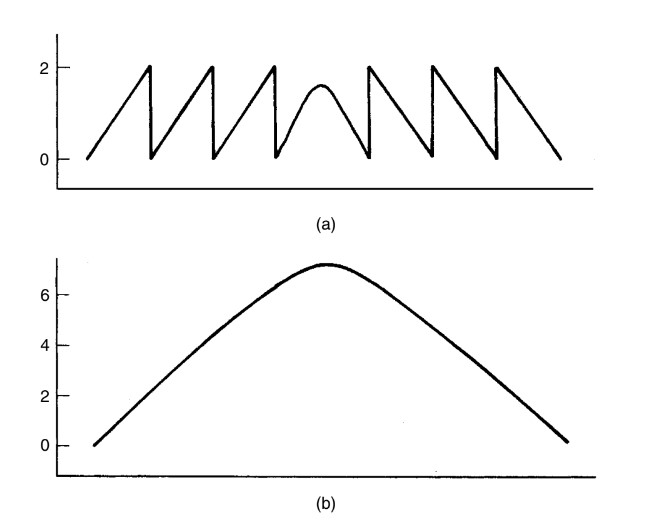
\includegraphics[width=0.25\textwidth]{Figures/UnwrappIlustration.jpg}
    \caption{(a) 'Saw-tooth’ wrapped phase function. (b) Phase function obtained by ‘unwrapping’ (a) \cite{gaasvik2003optical}}
    \label{fig:WRAPunwrap}
\end{figure}


\subsection{THREE DIMENSIONAL IMAGE RECONSTRUCTION}
After unwrapping is implemented successfully all is left a pure phase. This phase has encoded the depth measurements of the scanned object but also encodes information about the experimental parameters. In particular the angles formed by the camera and the scanned object $\beta$ (Figure \ref{fig:Exp_Setup}) and the spatial frequency of the fringes $w$.
%%FIGURA DE BETA Y W
In order to consider the experimental parameters in this model, Moire by fringe displacement puts forward a geometric relation between the phase $\phi$ and the topography of the object $z(x,y)$. Using 
\begin{equation}
    z = \frac{\phi}{2\pi} \frac{w}{tan(\beta)},
    \label{eq:topography}
\end{equation}
it is possible to decript the quantitative measurement of the scanned object. At any point of the scan, this technique will assign a z value. This information is stored in a matrix with dimensions specified by the photographs. 

% The beauty is in its simplicity. 
% Clever algorithmic implementations in Matlab
% Pasting two surfaces
